\chapter{Présentation et analyse des résultats}

\section{Déploiement de l'architecture finale}

L'architecture Médaillon définie en phase de conception a été intégralement
déployée dans Azure Data Lake Storage selon la hiérarchie suivante :

\begin{verbatim}
{conteneur_datalake}/
|-- bronze/
|   |-- {YYYY}/{MM}/    <- données mensuelles (ipf16.csv, capitaux, primes...)
|   |-- ref/            <- référentiels stables (ISIC, NAF, FFB, IRD Risk, SIRET)
|-- silver/
|   |-- {YYYY}/{MM}/    <- résultats intermédiaires par pipeline
|-- gold/
    |-- {YYYY}/{MM}/    <- Tables finales consommables par la BI
\end{verbatim}

Le partitionnement temporel (\texttt{\{YYYY\}/\{MM\}/}) permet un traitement
incrémental par vision mensuelle, en s'appuyant sur quarante-trois
\textit{file groups} configurés avec des schémas Spark stricts.

\section{Résultats d'exécution par pipeline analytique}

Au total, l'architecture produit \textbf{sept fichiers Delta Parquet distincts} par
vision mensuelle, répartis entre les tables Silver (intermédiaires) et Gold
(consolidations finales).

\vspace{0.3cm}
\noindent\fbox{
    \begin{minipage}{\textwidth}
        \vspace{0.2cm}
        \begin{center}
            {\large \textbf{Fichiers de sortie produits par vision mensuelle}}
        \end{center}
        \vspace{0.1cm}

        \begin{itemize}

            \item \textbf{PTF Mouvements}
            \begin{itemize}
                \item \textbf{Gold} : \texttt{ptf\_mvt\_{\{vision\}}}
                \item \textbf{Gold} : \texttt{ird\_risk\_q45\_{\{vision\}}}
                \item \textbf{Gold} : \texttt{ird\_risk\_q46\_{\{vision\}}}
                \item \textbf{Gold} : \texttt{ird\_risk\_qan\_{\{vision\}}}
            \end{itemize}

            \item \textbf{Capitaux}
            \begin{itemize}
                \item \textbf{Gold} : \texttt{az\_azec\_capitaux\_{\{vision\}}}
            \end{itemize}

            \item \textbf{Émissions}
            \begin{itemize}
                \item \textbf{Gold} : \texttt{primes\_emises\_{\{vision\}}\_pol}
                \item \textbf{Gold} : \texttt{primes\_emises\_{\{vision\}}\_pol\_garp}
            \end{itemize}

        \end{itemize}

        \vspace{0.2cm}
    \end{minipage}
}
\vspace{0.3cm}

\subsection{Pipeline PTF Mouvements}

Le pipeline PTF Mouvements consolide les mouvements de portefeuille AZ et AZEC,
applique les règles de filtrage métier, puis génère la table Gold utilisée pour les
analyses BI. Sur l’ensemble des visions testées, les volumes Python et SAS sont
strictement identiques, aussi bien en nombre total de polices qu’en répartition
par pôle et par code produit.

La vision 202512 sert d'exemple illustratif. La distribution par pôle obtenue
est identique entre les deux systèmes :

\begin{table}[H]
    \centering
    \caption{Distribution du portefeuille par pôle (exemple : vision 202512)}
    \label{tab:distrib_ptf}
    \begin{tabularx}{\textwidth}{|l|l|X|X|X|}
        \hline
        \textbf{Pôle} & \textbf{Canal} & \textbf{Python} & \textbf{SAS} & \textbf{Écart} \\
        \hline
        Pôle 1 (Agent)      & AZ          & 32 319 & 32 319 & 0,00\% \\
        \hline
        Pôle 3 (Courtage)   & AZ + AZEC   & 54 693 & 54 693 & 0,00\% \\
        \hline
        \textbf{Total}       &             & \textbf{87 012} & \textbf{87 012} & \textbf{0,00\%} \\
        \hline
    \end{tabularx}
\end{table}

\subsection{Pipeline Capitaux}

Le pipeline Capitaux applique l’indexation financière FFB et consolide les données
AZ et AZEC dans une table unique. Sur toutes les visions testées, les volumes Python
correspondent exactement aux volumes SAS et les indicateurs métier
(\texttt{VALUE\_INSURED}, \texttt{RISQUE\_DIRECT}) présentent une parité totale.

\subsection{Pipeline Émissions}

Le pipeline Émissions applique les règles métier sur les primes issues de One BI
puis génère deux tables Gold (par police et par garantie). Sur l'ensemble des
visions testées, les volumes et indicateurs Python (\texttt{Primes\_N},
\texttt{Primes\_X}, \texttt{MTCOM\_X}) sont strictement identiques à la
référence SAS.

\section{Bilan de la validation de parité}

La validation a été conduite sur plusieurs visions mensuelles et porte sur les
trois pipelines. Elle s’appuie sur trois niveaux de contrôle :

\begin{itemize}
    \item \textbf{Structure} : colonnes, types, schémas Spark, présence des champs obligatoires.
    \item \textbf{Volumes} : comparaison du nombre de polices par canal, par pôle et par code produit.
    \item \textbf{KPI métier} : comparaisons détaillées des indicateurs SAS vs Python.
\end{itemize}

L’ensemble des résultats détaillés est centralisé dans le fichier
\texttt{kpis\_results.xlsx} (Voir \hyperlink{annexe.F}{Annexe F}). Chaque feuille correspond à un pipeline et à une vision
mensuelle, et documente les écarts éventuels (colonnes \texttt{ECART}) ainsi que
les contrôles de cohérence par numéro de police.

Les tableaux \ref{tab:kpi_macro} et \ref{tab:kpi_micro} illustrent la structure des contrôles effectués. Le premier tableau présente le récapitulatif macroscopique garantissant qu'aucune police n'a été perdue ou dupliquée lors du traitement. Le second tableau détaille l'agrégation métier par code produit, permettant de vérifier la stricte équivalence des indicateurs au niveau granulaire.

\begin{table}[H]
    \centering
    \caption{Exemple de bilan de validation macroscopique (Cohérence des polices)}
    \label{tab:kpi_macro}
    \begin{tabularx}{\textwidth}{|l|l|X|X|r|}
        \hline
        \textbf{Indicateur} & \textbf{Canal} & \textbf{SAS} & \textbf{Python} & \textbf{Écart} \\
        \hline
        Nombre de polices & Agent & 32 319 & 32 319 & 0 \\
        \hline
        Nombre de polices & Courtage & 54 693 & 54 693 & 0 \\
        \hline
        Polices en différence & Total & 0 & 0 & 0 \\
        \hline
        Nombre de colonnes & Total & 110 & 110 & 0 \\
        \hline
        \textbf{Taux de différence global} & & & & \textbf{0,00\%} \\
        \hline
    \end{tabularx}
\end{table}

\begin{table}[H]
    \centering
    \caption{Exemple de validation au niveau granulaire (Nombre de polices par code produit)}
    \label{tab:kpi_micro}
    \begin{tabularx}{0.8\textwidth}{|X|r|r|r|}
        \hline
        \textbf{CDPROD} & \textbf{SAS (NBPTF)} & \textbf{Python (NBPTF)} & \textbf{Écart} \\
        \hline
        00023 & 14 & 14 & 0 \\
        \hline
        00024 & 444 & 444 & 0 \\
        \hline
        00526 & 12 & 12 & 0 \\
        \hline
        \dots & \dots & \dots & \dots \\
        \hline
        00559 & 147 & 147 & 0 \\
        \hline
        00616 & 5 & 5 & 0 \\
        \hline
        01054 & 1 118 & 1 118 & 0 \\
        \hline
    \end{tabularx}
\end{table}

Sur toutes les visions testées, les indicateurs calculés par Python sont
\textbf{strictement identiques} à ceux obtenus par SAS. Au-delà de l'exemple du tableau précédent, cette équivalence parfaite a été rigoureusement confirmée pour l'ensemble des indicateurs critiques de chaque pipeline :
\begin{itemize}
    \item \textbf{Mouvements de portefeuille} : affaires nouvelles (\texttt{NBAFN}), résiliations (\texttt{NBRES}), polices en vigueur (\texttt{NBPTF}) et décompte des polices (\texttt{NOPOL}).
    \item \textbf{Capitaux} : valeurs assurées (\texttt{VALUE\_INSURED}) et risques directs (\texttt{RISQUE\_DIRECT}).
    \item \textbf{Émissions} : totaux des primes émises (\texttt{Primes\_N}, \texttt{Primes\_X}) et commissions (\texttt{MTCOM\_X}).
\end{itemize}

Aucun écart n’est constaté, que ce soit sur les volumes, les distributions ou les KPI métier. Cette parité totale confirme la fidélité de l’implémentation Python par rapport au comportement SAS.

\section{Analyse qualitative du code produit}

\subsection{Modularité et réutilisabilité}

Le code Python a été structuré de manière modulaire afin de faciliter sa maintenance
et sa réutilisation dans d’autres marchés du programme SAS EXIST. Le module
\texttt{src/reader.py} est générique et lit automatiquement les file groups définis
dans \texttt{reading\_config.json}, tandis que les transformations sont
factorisées dans \texttt{utils/transformations/}.

\subsection{Configuration externalisée}

Les paramètres métier (file groups, règles de filtrage, mappings, schémas) sont
intégralement externalisés dans des fichiers JSON et des définitions Spark
centralisées. Cela permet d’adapter le comportement du pipeline sans modifier le
code Python, ce qui améliore fortement la maintenabilité.

\subsection{Comparaison qualitative SAS vs Python}

\vspace{0.3cm}
\noindent\fbox{
    \begin{minipage}{\textwidth}
        \vspace{0.2cm}
        \begin{center}
            {\large \textbf{Comparaison qualitative : SAS vs Python}}
        \end{center}
        \vspace{0.1cm}
        \begin{itemize}
            \item \textbf{Versionnement et documentation}
            \begin{itemize}
                \item SAS : versionnement manuel, documentation limitée.
                \item Python : version Git complet (Voir \hyperlink{annexe.G}{Annexe G}), documentation technique + fonctionnelle.
            \end{itemize}

            \item \textbf{Modularité}
            \begin{itemize}
                \item SAS : macros monolithiques difficilement extensibles.
                \item Python : modules isolés, configuration externalisée.
            \end{itemize}

            \item \textbf{Traçabilité et testabilité}
            \begin{itemize}
                \item SAS : logs peu détaillés, tests complexes.
                \item Python : logs structurés, contrôles automatiques, exécution distribuée via Spark.
            \end{itemize}
        \end{itemize}
        \vspace{0.2cm}
    \end{minipage}
}
\vspace{0.3cm}

\subsection{Comparaison des temps d'exécution et perspectives de scalabilité}

Outre l'exactitude des résultats, la migration vers PySpark a eu un impact significatif sur les performances. Pendant les tests, l'exécution complète du code Python sur l'environnement de développement (restreint à une machine virtuelle avec \textbf{8 Go de RAM} allouée) s'est achevée en \textbf{9 minutes} en moyenne. Sur le même périmètre et volume de données, l'environnement SAS mettait en moyenne \textbf{17 minutes}. Le temps de traitement a donc été divisé par près de deux, même avec des ressources matérielles contraintes.

Cette réduction immédiate du temps d'exécution n'est pourtant qu'une première étape. En effet, l'objectif du groupe à l'horizon 2028 est de basculer intégralement l'exécution sur \textbf{Azure Databricks}. Cette transition permettra au code (déjà écrit en PySpark et totalement compatible) d'exploiter la \textbf{scalabilité horizontale} des clusters. Le calcul pourra ainsi être distribué sur de multiples \textit{workers} (nœuds/machines) disposant de capacités de mémoire RAM beaucoup plus importantes. Cette future architecture débloquera des temps de traitements bien plus rapides, ouvrant la voie à des visions croisées sur plusieurs années ou à des réexécutions historiques massives, des opérations inenvisageables avec l'infrastructure SAS actuelle.

\begin{figure}[H]
\centering
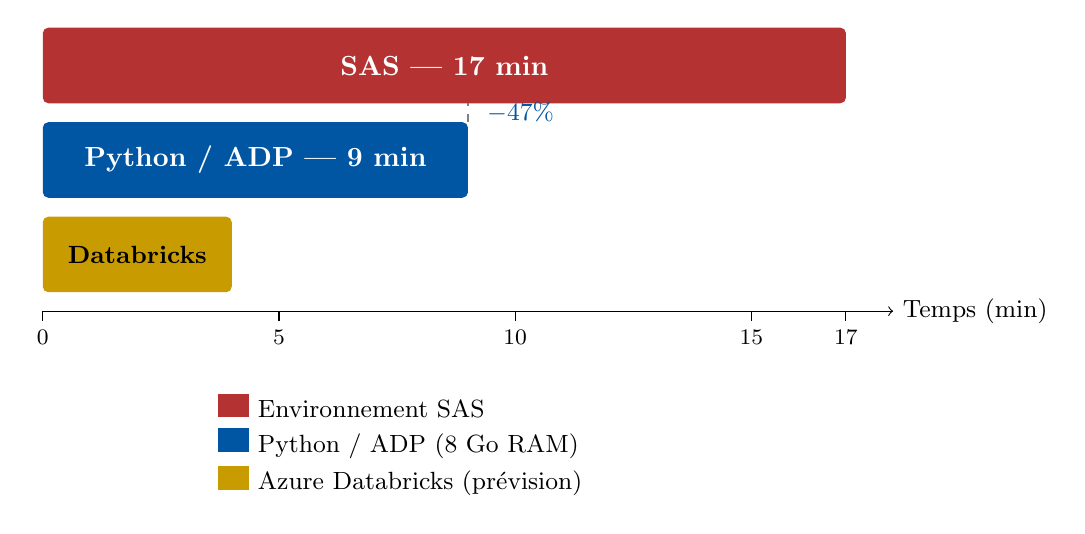
\begin{tikzpicture}[x=0.6cm, y=1.2cm]
    % Couleurs
    \definecolor{colorSAS}{RGB}{180,50,50}
    \definecolor{colorPy}{RGB}{0,86,163}
    \definecolor{colorDB}{RGB}{200,155,0}

    % Barre SAS (17 min)
    \fill[colorSAS, rounded corners=2pt] (0,2.0) rectangle (17,2.8);
    \node[white, font=\bfseries] at (8.5,2.4) {SAS — 17 min};

    % Barre Python/ADP (9 min)
    \fill[colorPy, rounded corners=2pt] (0,1.0) rectangle (9,1.8);
    \node[white, font=\bfseries] at (4.5,1.4) {Python / ADP — 9 min};

    % Barre Databricks (estimé)
    \fill[colorDB, rounded corners=2pt] (0,0.0) rectangle (4,0.8);
    \node[black, font=\bfseries\small] at (2.0,0.4) {Databricks};

    % Axe horizontal
    \draw[->] (0,-0.2) -- (18,-0.2) node[right, font=\small] {Temps (min)};
    \foreach \x in {0,5,10,15,17}{
        \draw (\x,-0.2) -- (\x,-0.3) node[below, font=\footnotesize] {\x};
    }

    % Annotation gain
    \draw[dashed, gray] (9,1.8) -- (9,2.0);
    \node[right, font=\small, colorPy] at (9.2, 1.9) {\textbf{$-47\%$}};

    % Légende (verticale centrée sous le graphe)
    \begin{scope}[shift={(3.5,-1.2)}]
        \node[right, font=\small] at (0,0) {\textcolor{colorSAS}{\rule{0.4cm}{0.3cm}} Environnement SAS};
        \node[right, font=\small] at (0,-0.4) {\textcolor{colorPy}{\rule{0.4cm}{0.3cm}} Python / ADP (8 Go RAM)};
        \node[right, font=\small] at (0,-0.8) {\textcolor{colorDB}{\rule{0.4cm}{0.3cm}} Azure Databricks (prévision)};
    \end{scope}
\end{tikzpicture}
\caption{Comparaison des temps d'exécution moyens par vision mensuelle}
\label{fig:perf_comparison}
\end{figure}